\section{The Scaling Hypothesis}

Discussing the realations between critical exponents is a foundamental step in the study and comprehension of critical phenomena. The scaling hypothesis is a powerful tool that allows us to derive these relations and understand the behavior of physical quantities near the critical point.

We can start by considering the free energy per unit volume \(f(t,h) = F(t,h)/V\) as computed via the saddle point approximation in the Landau-Ginzburg theory, which is given by
\[
    f(t,h) = \text{min}_m \left[ \frac{t}{2}m^2 + u m^4 - h m \right] = \begin{dcases}
        - \frac{1}{16} \frac{t^2}{u}               & (h=0,\,t < 0),      \\
        -\frac{3}{4^{4/3}} \frac{h^{4/3}}{u^{1/3}} & (h \neq 0,\,t = 0), \\
    \end{dcases}
\]
where these singularities of the free energy density \(f\)\footnote{There is a jump discontinuity (at \(t>0\) we have that \(f=0\)), and also higher order derivatives of \(f\) with respect to \(h\) (such as the magnetic susceptibility) or \(t\) are discontinuous at \(t=0\).} at the critical point are consistent with the assumption that the free energy density \(f\) is a \textbf{generalized homogeneous function} of the reduced temperature \(\vert t \vert\) and the external field \(h\) when we study it close to the critical point \(T_c\) (as we will soon show). This is a non-trivial assumption, which is not satisfied by the mean field theory, but it is satisfied by the true free energy density \(f\) of the system, which can be very different from the one predicted by the mean field theory. The scaling hypothesis is based on this homogeneity assumption, which allows us to derive scaling relations between critical exponents.

Let us start by understanding the mathematical definition of a generalized homogeneous function.

\begin{definition}[Homogeneous function]
    A function \(f\,:\,\mathbb{R}^n \to \mathbb{R}\) is called a homogeneous function of degree \(k\) if it satisfies the following scaling property:
    \[
        f(\lambda x_1, \lambda x_2, \dots, \lambda x_n) = \lambda^k f(x_1, x_2, \dots, x_n), \quad \forall \lambda > 0.
    \]
    This means that if we scale all the input variables by a factor of \(\lambda\), the output of the function scales by a factor of \(\lambda^k\). The degree \(k\) can be any real number, and it characterizes how the function responds to scaling transformations. It is called the \textbf{degree of homogeneity}.
\end{definition}

\begin{definition}[Generalized homogeneous function]
    A function \(f\,:\,\mathbb{R}^n \to \mathbb{R}\) is called a generalized homogeneous function if there exist real numbers \(d_1, d_2, \dots, d_n\, \in \mathbb{R}\) such that it satisfies the following scaling property:
    \[
        f(\lambda^{d_1} x_1, \lambda^{d_2} x_2, \dots, \lambda^{d_n} x_n) = \lambda f(x_1, x_2, \dots, x_n), \quad \forall \lambda > 0.
    \]
    In this case, the function scales linearly with respect to the scaling of its arguments, but each argument can scale with a different exponent \(d_i\). The exponents \(d_i\) characterize how each variable contributes to the overall scaling behavior of the function.

\end{definition}

Now taking a generalized homogeneous function of two variables \(f(x,y)\) such that:
\[
    f(\lambda^{d_1} x, \lambda^{d_2} y) = \lambda f(x,y),
\]
if we set
\[
    \lambda = \left(\frac{1}{x}\right)^{\frac{1}{d_1}},
\]
we can notice how the function \(f\) can be rewritten as
\[
    f(1, \frac{1}{x^{d_2/d_1}} y) = \left(\frac{1}{x}\right)^{\frac{1}{d_1}} f(x,y).
\]
Now if we define \(g(z)=f(1,z)\), we can invert the relation above to obtain
\[
    f(x,y) = x^{1/d_1} g\left(\frac{y}{x^{d_2/d_1}}\right),
\]
which therefore shows how the generalized homogeneous function \(f\) can be expressed in terms of a single variable, which is the ratio \(\frac{y}{x^{\Delta}}\) (where \(\Delta = \frac{d_2}{d_1}\)) of the two original variables, up to an overall prefactor \(x^{d_1}\). This is the essence of the scaling hypothesis, which states that near the critical point, physical quantities can be expressed as homogeneous functions of the relevant variables, leading to scaling relations between critical exponents; we will see this more explicitly in the following.

If we assume that \uline{the true free energy density \(f\) is a generalized homogeneous function} of the reduced temperature \(\vert t \vert\) and the external field \(h\) when we study it close to the critical point \(T_c\), then it must satisfy the following scaling property:
\[
    f(\vert t \vert, h) = \vert t \vert^{d} g\left(\frac{h}{\vert t \vert^{\Delta}}\right),
\]
for some \(d\), \(\Delta\) and \(g\) (notice how we are now treating \(d\) and \(\Delta\) as independent parameters). In general, the true free energy density \(f\) of the system can be very different from the one predicted by the mean field theory.

\begin{remark}
    It has to be clarified that we are considering only the singular part of the free energy density \(f\) in the homogeneity assumption, since the regular part of \(f\) does not contribute to the singularities of physical quantities at criticality.
\end{remark}

Knowing the singularities of the free energy density \(f(t,h)\), we can fix the values of \(d\) and \(\Delta\) and therefore derive the scaling relations between critical exponents. Thus we can start from the singularities of the free energy density \(f\) as predicted by the saddle point approximation in the Landau-Ginzburg theory, and see how they are consistent with the homogeneity assumption that we made on the free energy density \(f\).
\begin{itemize}
    \item For \((h=0,\,t\neq 0)\), we must have
          \[
              f(t,0) \sim \frac{\vert t \vert^2}{u}, \quad \implies \quad d = 2,
          \]
          where we used the limit
          \[
              \lim_{x \to 0} g(x) \sim \frac{1}{u}.
          \]
    \item Instead, for \((h\neq 0,\,t \to 0)\), we must have
          \[
              \lim_{t \to 0} f(t,h) \sim \frac{h^{4/3}}{u^{1/3}},
          \]
          which can be verified by setting
          \[
              \lim_{x \to \infty} g(x) \sim \frac{x^{4/3}}{u^{1/3}}.
          \]
          Now, using the last relation, we can fix the value of \(\Delta\) as follows:
          \[
              \lim_{t \to 0} f(t,h) \sim \vert t \vert^2 \frac{h^{4/3}}{u^{1/3} \, t^{4\Delta/3}} \quad \implies \quad \Delta = \frac{3}{2}.
          \]
\end{itemize}
We can conclude that the homogeneity assumption in the singular part of the free energy density \(f\) is consistent with the singularities predicted by the saddle point approximation, with
\[
    d = 2, \quad \Delta = \frac{3}{2}.
\]

We can now state the \textbf{scaling hypothesis} as follows: \textit{going beyond the saddle point approximation, the singular part of the free energy density \(f\) remains a generalized homogeneous function of the reduced temperature \(\vert t \vert\) and the external field \(h\) when we study it close to the critical point \(T_c\)}. This is a non-trivial assumption, which is not satisfied by the mean field theory, but it is satisfied by the true free energy density \(f\) of the system, which can be very different from the one predicted by the mean field theory.

\subsection{Scaling Relations}

Assuming thus that the singular part of the free energy density \(f\) is a generalized homogeneous function of the reduced temperature \(\vert t \vert\) and the external field \(h\) when we study it close to the critical point \(T_c\), we can again write
\[
    f(\vert t \vert, h) = \vert t \vert^{d} g\left(\frac{h}{\vert t \vert^{\Delta}}\right),
\]
for some \(d\), \(\Delta\) and \(g\). This does not imply the free energy of the mean field theory, which is a particular approximation of the true free energy (which can even have this form in general, but with different exponents), but it is a more general assumption that we make on the true free energy itself. Let us now find a way to relate the exponents \(d\) and \(\Delta\) to the critical exponents.

\subsubsection{Critical Exponents: \(\alpha\)}

We start by relating \(d\) with the critical exponent \(\alpha\) that describes the singularity of the heat capacity \(C\) at the critical point. We know that
\[
    C \propto - \frac{\partial^2 f}{\partial t^2},
\]
so that we have to compute the second derivative of the free energy density \(f\) with respect to the temperature \(T\). Computing the first derivative of \(f\) with respect to \(T\):
\[
    \begin{aligned}
        \frac{\partial f}{\partial t} & \sim d \vert t \vert^{d-1} g\left(\frac{h}{\vert t \vert^{\Delta}}\right) - \Delta \vert t \vert^{d-\Delta-1} h g^{\prime}\left(\frac{h}{\vert t \vert^{\Delta}}\right)                  \\
                                      & = \vert t \vert^{d-1} \left[ d\,g\left(\frac{h}{\vert t \vert^{\Delta}}\right) - \Delta \frac{h}{\vert t \vert^{\Delta}} g^{\prime}\left(\frac{h}{\vert t \vert^{\Delta}}\right) \right] \\
                                      & = \, : \vert t \vert^{1-\alpha} \tilde{g}\left(\frac{h}{\vert t \vert^{\Delta}}\right),
    \end{aligned}
\]
since in the previous computation \(h\) appeared always divided by \(\vert t \vert^{\Delta}\), in order to let us define the function \(\tilde{g}\).

\begin{remark}
    More generally, partial derivative of an generalized homogeneous function will again be an generalized homogeneous function, with different prefactors and a different functional form \(\tilde{g}\) (which is related to the original function \(g\) by differentiation).
\end{remark}

Repeating the same procedure to compute the second derivative of \(f\) with respect to \(T\), we obtain
\[
    C \propto - \frac{\partial^2}{\partial t^2} f \sim \vert t \vert^{-\alpha} \tilde{\tilde{g}}\left(\frac{h}{\vert t \vert^{\Delta}}\right),
\]
where \(\tilde{\tilde{g}}\) is another appropritely defined function.

Now, since we need the critical exponent \(\alpha\) to describe the singularity of the heat capacity \(C\) at the critical point in absence of external field \(h\), we need to have
\[
    C(t, h=0) \xrightarrow{t \to 0} \vert t \vert^{-\alpha} \tilde{\tilde{g}}(0) = \text{const} \cdot \vert t \vert^{-\alpha}.
\]
Therefore, we can conclude that the critical exponent \(\alpha\) is related to the exponent \(d\) by the following relation:
\[
    \lim_{x \to 0} \tilde{\tilde{g}}(x) = \text{const} \implies \alpha = 2 - d,
\]
and thus we found the relation between the critical exponent \(\alpha\) and the exponent \(d\) that appears in the homogeneity assumption of the free energy density \(f\): \(d = 2 - \alpha\). The logic behind this is that we need to now how this function behaves at the critical point, where it could go to 0, diverge to infinity or go to a constant; since
\[
    \lim_{t \to 0} C (t, h=0) \sim \vert t \vert^{-\alpha},
\]
then we need to have \(\lim_{x \to 0} \tilde{\tilde{g}}(x) = \text{const}\) in order to have the correct singularity of the heat capacity \(C\) at the critical point.

\subsubsection{Critical Exponents: \(\beta\)}

Now the only unknown parameter is \(\Delta\), which we call the \textbf{gap exponent}: it is related to the critical exponent \(\beta\) that describes the singularity of the order parameter \(m\) at the critical point. We are saying that the theory in which we compute the critical exponent \(\beta\) is not important (mean field, Landau-Ginzburg, etc), but it is important that the true free energy density \(f\) has the homogeneity property that we assumed above, with some value of \(\Delta\). Thus let us relate \(\Delta\) to \(\beta\) by computing the order parameter \(m\) as a function of the reduced temperature \(t\) at zero external field \(h=0\): remember the definition of the critical exponent \(\beta\) is
\[
    m(t,h=0) \sim \vert t \vert^{\beta},
\]
then we can compute \(m\) by taking the derivative of the free energy density \(f\) with respect to the external field \(h\):
\[
    m = - \frac{\partial f}{\partial h} \sim \vert t \vert^{d-\Delta} g^{\prime} \left(\frac{h}{\vert t \vert^{\Delta}}\right),
\]
and therefore we can conclude that the critical exponent \(\beta\) is related to the gap exponent \(\Delta\) by the following relation:
\[
    \lim_{x \to 0} g^{\prime}(x) = \text{const} \implies \beta = d - \Delta,
\]
which is the second scaling relation that we were looking for
\[
    \beta = d - \Delta = 2 - \alpha - \Delta.
\]

\subsubsection{Critical Exponents: \(\delta\)}

Now we can consider the critical exponent \(\delta\), which describes the singularity of the order parameter \(m\) at the critical point as a function of the external field \(h\):
\[
    m(t=0,h) \sim h^{1/\delta},
\]
then we can assume that the function \(g\) behaves as
\[
    \lim_{x \to \infty} g(x) \sim x^{p+1}, \quad \implies \quad \lim_{x \to \infty} g^{\prime}(x) \sim x^p,
\]
which is the only reasonable behavior that we can assume for the function \(g\) in order to have a power law singularity of the order parameter \(m\) at the critical point. Therefore, we can compute the order parameter \(m\) at the critical point \(t=0\) as a function of the external field \(h\):
\[
    \lim_{t \to 0} m(t,h) \sim \vert t \vert^{2-\alpha-\Delta} \left(\frac{h}{\vert t \vert^{\Delta}}\right)^{p},
\]
which is well-defined only if \(p \Delta = 2 - \alpha - \Delta\) leading us to
\[
    \lim_{t \to 0} m(t,h) \sim h^{\frac{2-\alpha-\Delta}{\Delta}},
\]
which recalling the definition of the critical exponent \(\delta\) leads us to the following scaling relation:
\[
    \delta = \frac{\Delta}{2-\alpha-\Delta} = \frac{\Delta}{\beta}.
\]

\subsubsection{Critical Exponents: \(\gamma\)}

For the susceptibility \(\chi\), we can use the same arguments and procedures, computing it as the derivative of the magnetization \(m\) with respect to the external field \(h\):
\[
    \chi(t,h) \propto \frac{\partial m}{\partial h} = - \frac{\partial^2 f}{\partial h^2} \sim \vert t \vert^{2-\alpha-2\Delta} g^{\prime \prime}\left(\frac{h}{\vert t \vert^{\Delta}}\right),
\]
which, after making the usual assumptions on the behavior of the function \(g\) as before, leads us to
\[
    \chi(t,h=0) \sim \vert t \vert^{2-\alpha-2\Delta}, \quad \chi(t=0,h) \sim \vert t \vert^{-\gamma},
\]
obtaining, from the previous definition of the critical exponent \(\gamma\), the following scaling relation:
\[
    \gamma = 2\Delta + \alpha - 2.
\]

\subsubsection{Scaling Identities}

After these computations, we have found the following scaling relations between critical exponents:
\[
    \begin{dcases}
        \alpha = 2 - d,                                                 \\
        \beta = d - \Delta = 2 - \alpha - \Delta,                       \\
        \delta = \frac{\Delta}{\beta} = \frac{\Delta}{2-\alpha-\Delta}, \\
        \gamma = \Delta - \beta = 2\Delta + \alpha - 2,
    \end{dcases}
\]
showing how the gap exponent \(\Delta\) appear in all the expressions for the critical exponents: it is a fundamental exponent that characterizes the scaling behavior of the free energy density \(f\) and it is related to all the critical exponents.

Since we have only two unknown parameters \(d\) and \(\Delta\), we can express all the critical exponents in terms of these two parameters, and therefore we can derive scaling identities between critical exponents by eliminating \(d\) and \(\Delta\) from the previous relations.

For example, from the scaling relations of \(\beta\), \(\delta\) and \(\gamma\), we can derive the following scaling identities:
\[
    \begin{dcases}
        \alpha + 2\beta + \gamma = 2,      & \textbf{Rushbrooke's identity,} \\
        \delta - 1 = \frac{\gamma}{\beta}, & \textbf{Widom's identity.}      \\
    \end{dcases}
\]
Now, the first identity is simply obtained by summing the expressions of \(\alpha\), \(2\beta\) and \(\gamma\); the second one, by direct computation we have:
\[
    \delta - 1 = \frac{\Delta}{\beta} - 1 = \frac{\Delta - 2 + \alpha + \Delta}{\beta},
\]
and by recalling the expression of \(\gamma\) we can rewrite the previous expression as
\[
    \delta - 1 = \frac{2\Delta + \alpha - 2}{\beta} = \frac{\gamma}{\beta}.
\]

These relations can be tested experimentally and numerically, and they are indeed satisfied with good precision, despite the fact that the individual exponents are different than the one predicted by the mean field theory.

\begin{table}[H]
    \centering
    \setlength{\tabcolsep}{16pt}
    \begin{tabular}{c c c c c c}
        \toprule
        $\alpha$ & $\beta$ & $\gamma$ & $\delta$ & $\nu$  & $\eta$ \\
        \midrule
        $0.11$   & $0.32$  & $1.24$   & $4.9$    & $0.63$ & $0.04$ \\
        \bottomrule
    \end{tabular}
    \caption{Critical exponents for the three-dimensional Ising model, which is a paradigmatic example of an uniaxial ferromagnet. These exponents are different from the ones predicted by the mean field theory, but they satisfy the scaling identities with precision.}
    \label{tab:critical_exponents_uniaxial_ferromagnet_3d}
\end{table}

So it seems that even in systems with very different exponents, the scaling relations are still satisfied, which is a strong evidence in favor of the scaling hypothesis and the homogeneity assumption that we made on the true free energy density \(f\). Historically, these identities and relations among critical exponents were derived experimentally and numerically before the scaling hypothesis was formulated, which in the end explains their universal validity.

\subsection{Hyperscaling Hypothesis}

The homogeneity assumption do not apply only to the free energy density \(f\), but also to other physical quantities derived from it. But it says nothing about the correlation functions. In order to obtain identities related to exponents of the correlation functions, we need to make two additional assumptions which will seem to be more foundamental and more general than the homogeneity assumption on the free energy density \(f\): the \textbf{hyperscaling hypothesis}.
\begin{itemize}
    \item The correlation length \(\xi\) is a generalized homogeneous function of the reduced temperature \(\vert t \vert\) and the external field \(h\) when we study it close to the critical point \(T_c\):
          \[
              \xi(t,h) = \vert t \vert^{-\nu} g\left(\frac{h}{\vert t \vert^{\Delta}}\right).
          \]
    \item Close to criticality, \(\xi\) is the most important lenght scale in the system and is solely responsible for the singular contributions to thermodynamic quantities.
\end{itemize}

The idea is now to show euristically how to use these assumptions to derive the scaling form of the free energy density \(f\) and therefore the scaling relations between critical exponents.

\begin{figure}[H]
    \begin{minipage}{0.55\textwidth}
        \centering
        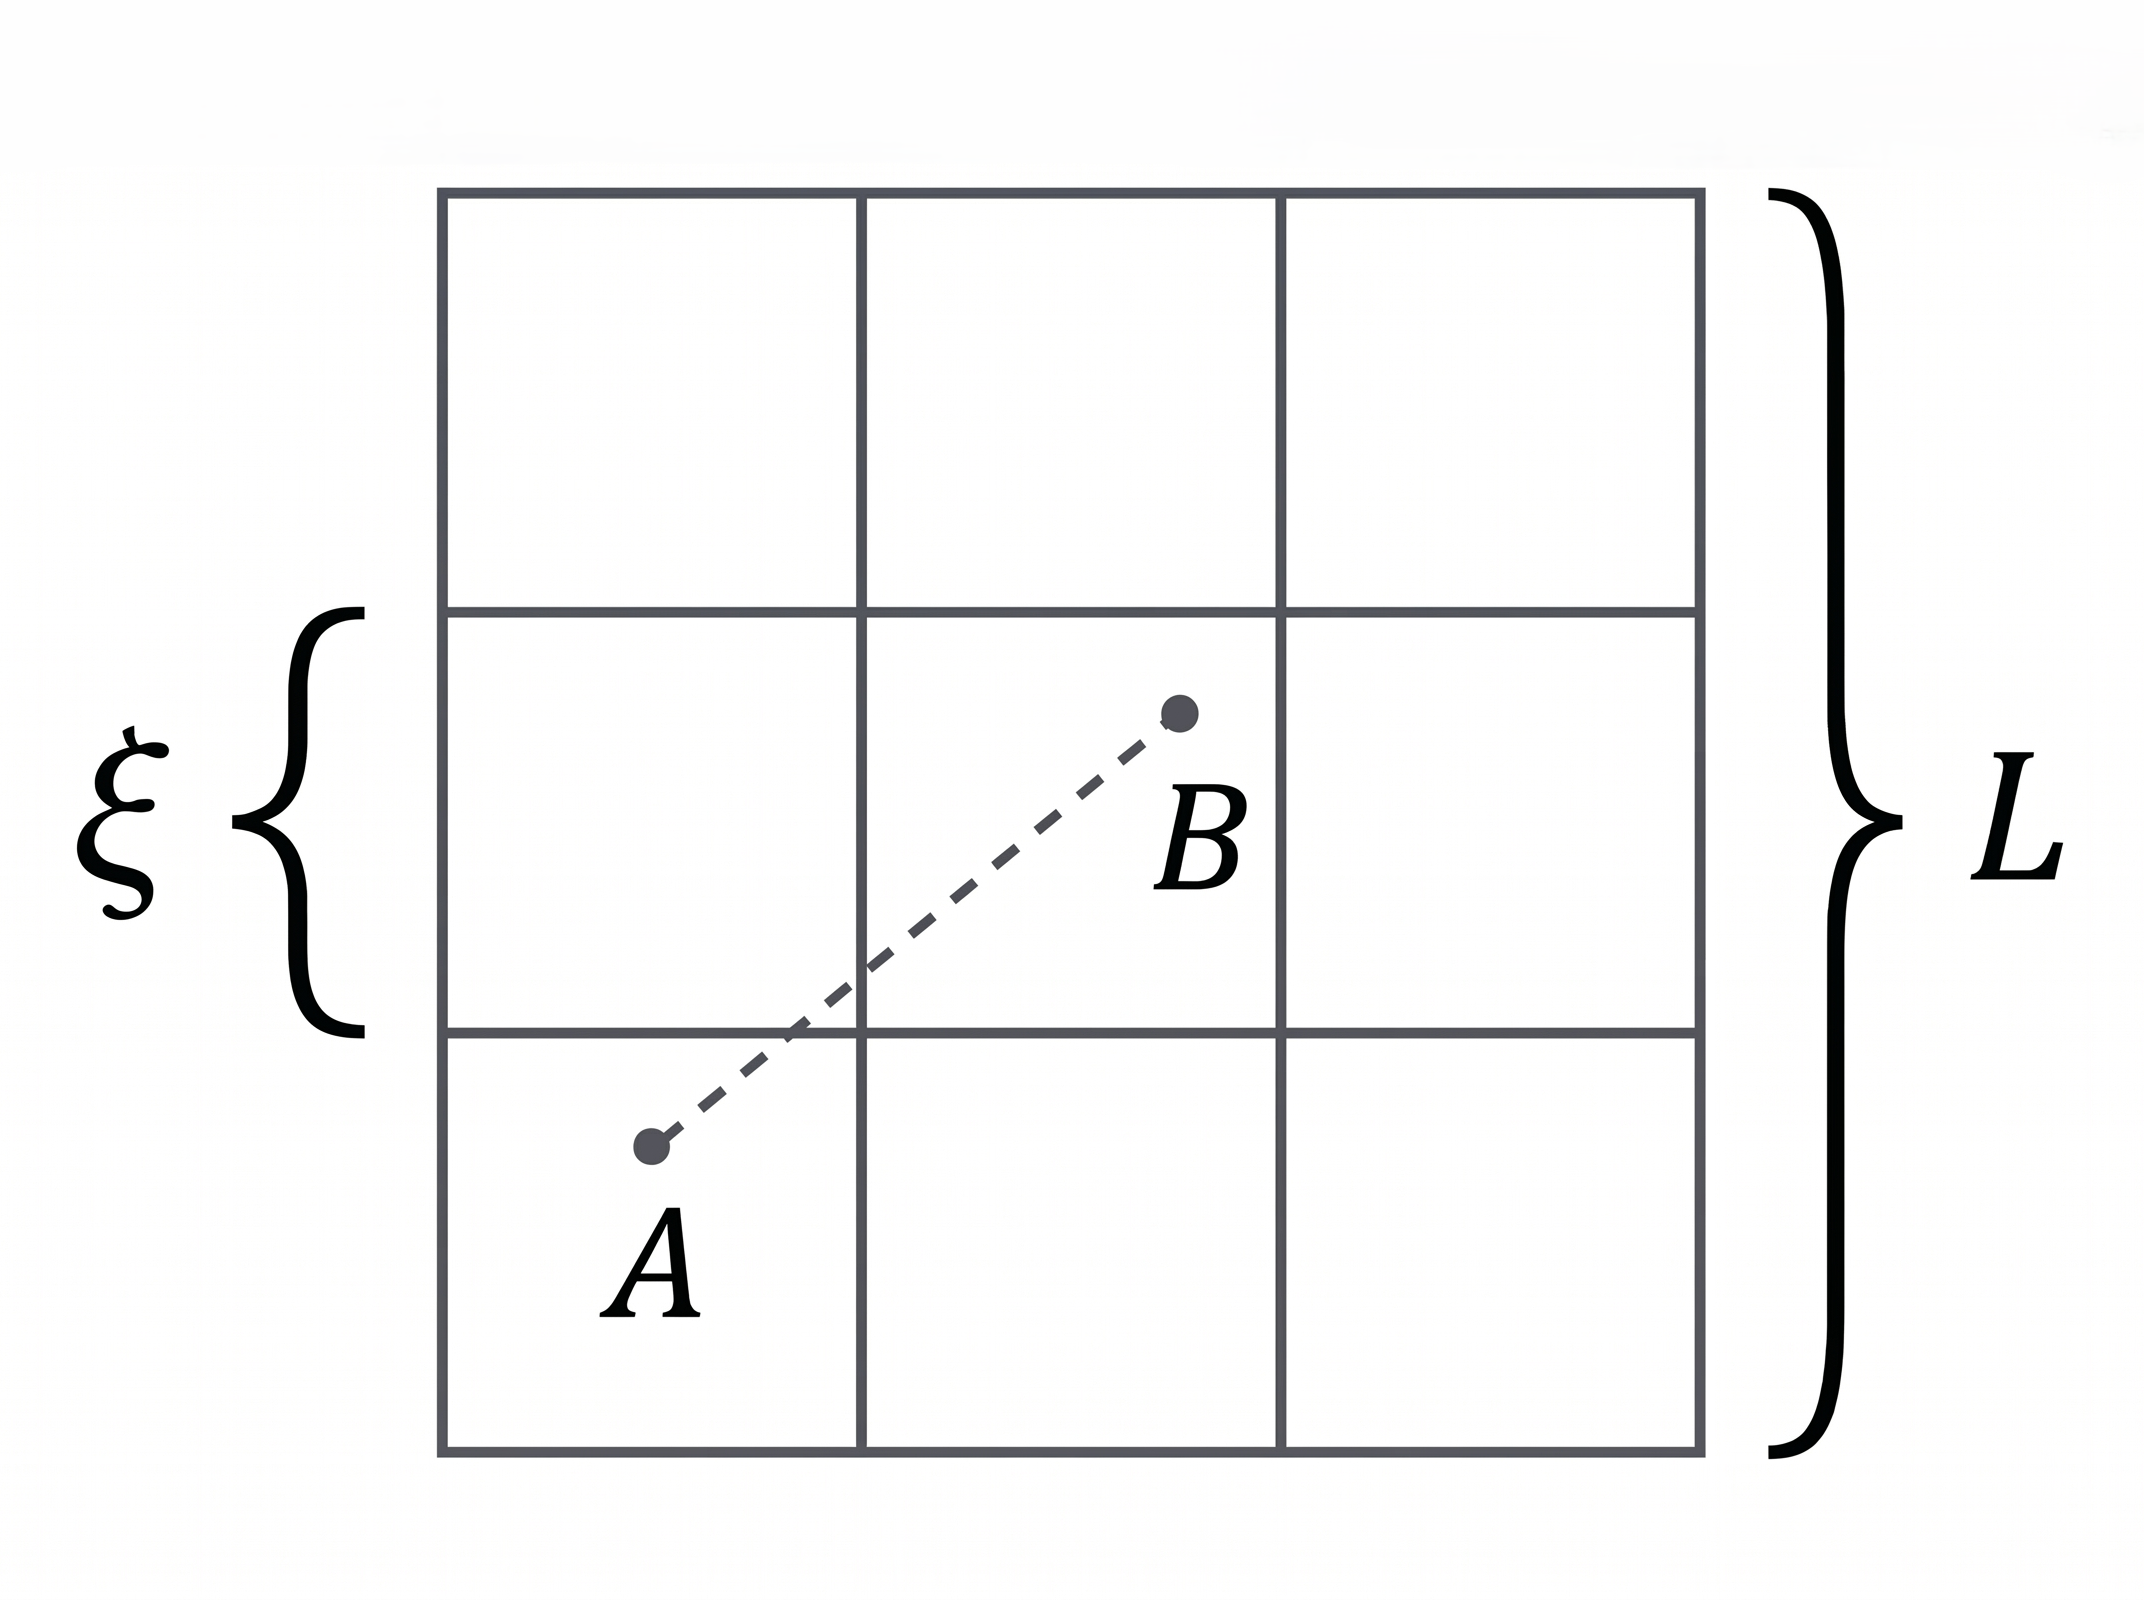
\includegraphics[width=0.7\textwidth]{img/hyperscaling.png}
        \caption{The system can be divided into blocks of linear size \(\xi\) and volume \(\xi^d\), so that we have \(N_b = V/\xi^d\) uncorrelated subsystems in total.}
    \end{minipage}
    \hfill
    \begin{minipage}{0.4\textwidth}
        We can start by considering a system of linear size \(L\) and volume \(V = L^d\), where \(d\) is the spatial dimension of the system. We can divide the system into blocks of linear size \(\xi\) and volume \(\xi^d\), so that we have \(N_b = V/\xi^d\) blocks in total.

        Now, since we are assuming that \(\xi\) is the most important length scale in the system, we can assume that each block contributes independently to the free energy density \(f\), so that points from different blocks can be considered uncorrelated.
    \end{minipage}
\end{figure}

Since we are interested in the computation of the free energy density \(f\), we can start from the \textbf{partition function} \(\mathcal{Z}\) of the system: up to a first approximation (if we are interested only in the diverging behavior of \(\mathcal{Z}\)), we can write the partition function \(\mathcal{Z}\) as a sum of local partition functions
\[
    \log \mathcal{Z} \sim \left(\frac{L}{\xi}\right)^d g_s,
\]
where \(g_s\) is the single region contribution to the free energy, while the prefactor \((L/\xi)^d\) counts the number of uncorrelated blocks in the system. Furthermore, since \(\mathcal{Z}\) is dimensionless, we can assume that \(g_s\) is a dimensionless function.

Finally, since by the second assumption of the hyperscaling hypothesis we have that \(\xi\) is the only relevant length scale in the system, then it follows that any singular behavior of \(\log \mathcal{Z}\) must be due to the divergence of \(\xi\) at the critical point, so that \(g_s\) must be regular at the critical point, and therefore we can write
\[
    f(t,h) \sim \frac{1}{L^d} \log \mathcal{Z} \sim \xi^{-d} \sim \vert t \vert^{\nu d} g\left(\frac{h}{\vert t \vert^{\Delta}}\right),
\]
where the second equality is obtained close to criticality, while the last equality is obtained by using the homogeneity assumption on the correlation length \(\xi\) from the hyperscaling hypothesis.

Therefore, we have shown how to derive the scaling form of the free energy density \(f\) from the hyperscaling hypothesis, which is a more general and more fundamental assumption than the homogeneity assumption on the free energy density \(f\) itself.

\subsubsection{Hyperscaling Identities}

In addition, we get a new scaling relation between the critical exponent \(\alpha\) and the correlation length exponent \(\nu\): by equating the previous expression of the free energy density \(f\) with the one obtained from the homogeneity assumption, we get
\[
    2-\alpha = d \nu, \quad \textbf{Josephson's identity.}
\]
Identities like the one above are called \textbf{hyperscaling identities}, since they involve the spatial dimension \(d\) of the system,\footnote{When studying the scaling hypothesis, \(d\) was a generic parameter, now it is exactly the spatial dimension of the system.} and they are a direct consequence of the hyperscaling hypothesis. These identities are satisfied in low dimensions, but they are violated in high dimensions, where the mean field theory becomes exact and the critical exponents take their mean field values. Indeed, the previous relation among \(\alpha\) and \(\nu\) is satisfied by the real exponents in two or three dimensions (as one can see from the Table \ref{tab:critical_exponents_uniaxial_ferromagnet_3d}), however it does not agree with the saddle point (mean field) solution for \(d > 4\): in this case, the mean field theory becomes exact and the critical exponents take their mean field values, which do not satisfy the previous relation (indeed we would have \(\alpha=0\) and \(\nu = 1/2\)).

This is a strong evidence that the hyperscaling hypothesis is not valid in high dimensions, where the mean field theory becomes exact, while it is valid in low dimensions, where the critical exponents take non-mean field values. Any theory that aims to explain the critical behavior of systems must therefore satisfy the hyperscaling hypothesis in low dimensions, while taking into account its violation in high dimensions. This is one of the main challenges in the study of critical phenomena, and it is one of the reasons why the renormalization group theory is so important, since it provides a framework to understand the validity of the hyperscaling hypothesis and its violation in high dimensions.

Before embarking in the study of the renormalization group theory, we will first discuss the last critical exponent \(\eta\) that describes the singularity of the correlation function at the critical point.

\subsubsection{Correlation Functions and \(\eta\)}

The critical exponent \(\eta\) describes the singularity of the correlation function \(G(\mathbf{x})\) at the critical point; we already derived the connected correlation function \(G^c(\mathbf{x})\) keeping the second order corrections to the saddle point approximation in the Landau-Ginzburg theory. We found that at the critical point \(t=0\) the correlation lenght diverges \(\xi \to \infty\), obtaining
\[
    G^c(\mathbf{x}) = \langle \phi(\mathbf{x}) \phi(\mathbf{0}) \rangle \sim \frac{1}{\vert \mathbf{x} \vert^{d-2}}.
\]
We know this behavior to be correct in high dimensions (\(d\geq 4\) for ising, \(d \geq D_c\) in general), where the mean field theory becomes exact, but it is not correct in low dimensions, where the critical exponents take non-mean field values.

For \(d < 4\), the mean field result is not correct anymore. However, it is still true that at the critical point the correlation length diverges (\(\xi \to \infty\)). Because an exponential decay of the form \(e^{- \vert \mathbf{x} \vert / \xi}\) inherently requires a \textit{finite} length scale \(\xi\), the correlation function \(G(\mathbf{x})\) cannot decay exponentially at criticality.

Therefore, \(G(\mathbf{x})\) must still vanish for large distances \(\vert \mathbf{x} \vert \to \infty\) as a \textbf{power law}. We can account for the deviation from the mean field behavior by introducing a new critical exponent \(\eta\) as follows:
\[
    G(\mathbf{x}) \sim \frac{1}{\vert \mathbf{x} \vert^{d-2+\eta}}.
\]
This is the definition of the critical exponent \(\eta\), which describes the singularity of the correlation function at the critical point, and it is usually called the \textbf{anomalous dimension}.\footnote{The critical exponent \(\eta\) is related to the anomalous dimension of the field \(\phi\) in the renormalization group theory, and it is a measure of how much the correlation function deviates from the mean field behavior at the critical point.}

Now, even if we did not see this explicitly, it is easy to relate \(\chi\) the susceptibility to the connected correlation functions \(G^c(\mathbf{k})\) as follows:
\[
    \chi \sim \int \mathrm{d}^d \mathbf{x} \, G^c(\mathbf{x}),
\]
so that in the end we find that \(\eta\) can be related to the exponent appearing in the singularity of the susceptibility \(\chi\) at the critical point, \(\gamma\), since
\[
    \chi \sim \vert t \vert^{-\gamma}, \quad \text{as } t \to 0.
\]
Notice how the expression connecting the susceptibility to the correlation functions is valid only up to distances \(\sim \xi\), since for distances larger than \(\xi\) the correlation function \(G^c(\mathbf{x})\) vanishes exponentially.

We can now plug the previous expression of the correlation function \(G^c(\mathbf{x})\) at the critical point into the expression of the susceptibility \(\chi\) to obtain\footnote{Here, we have assumed that the connected correlation function, for values of \(\vert \mathbf{x} \vert \gg \xi\), is suppressed (as a power law), so that we can neglect its contribution in that regime.}
\[
    \chi \sim \int_0^{\xi} \mathrm{d}^d \mathbf{x} \, \frac{1}{\vert \mathbf{x} \vert^{d-2+\eta}} \sim \xi^{2-\eta} \sim \vert t \vert^{-\nu (2-\eta)},
\]
where we have used the critical behavior of the correlation length \(\xi\) at the critical point, given by
\[
    \xi \sim \vert t \vert^{-\nu}.
\]
Now, recalling the critical behavior of the susceptibility, we are lead to the following hyperscaling relation between the critical exponents \(\gamma\), \(\nu\) and \(\eta\):
\[
    \gamma = (2-\eta) \nu, \quad \textbf{Fisher's identity.}
\]
This is another hyperscaling identity, since it involves the critical exponent \(\nu\) that describes the divergence of the correlation length \(\xi\) at the critical point, and it is a direct consequence of the hyperscaling hypothesis. Again, this identity is satisfied in low dimensions, but it is violated in high dimensions, where the mean field theory becomes exact and the critical exponents take their mean field values.

\begin{remark}
    The scaling hypothesis is a general assumption that can be applied to a wide range of systems and phenomena, and gives us predictions (such as the scaling relations between critical exponents) that can be tested experimentally and numerically to be true for any value of the spatial dimension \(d\).

    The hyperscaling hypothesis is a more specific assumption which allows us to derive additional scaling relations to be used in order to derive the hyperscaling identities for the exponents \(\nu\) and \(\eta\). But this assumption gives correct predictions only in low dimensions, while it is violated in high dimensions, where the mean field theory becomes exact and the critical exponents take their mean field values.
\end{remark}

\subsubsection{Scale Invariance}

Until now, we have made more of a phenomenological analysis of the critical behavior of systems, by making assumptions on the form of the free energy density \(f\) and the correlation length \(\xi\) close to the critical point, and by deriving scaling relations between critical exponents from these assumptions. However, in the next chapter, we are going to introduce the renormalization group theory, which will provide us with a more fundamental and more microscopic understanding of the critical behavior of systems, and it will allow us to derive the scaling hypothesis and the hyperscaling hypothesis from first principles. So let us make some observations about the scale invariance of systems at criticality, which will be a key concept in the renormalization group theory.

A consequence of the previous scaling assumptions is that, at criticality, the system acquire an additional symmetry: the \textbf{dilatation symmetry}. Namely, under a change of scale, the critical correlation functions transform as
\[
    G(\lambda \mathbf{x}) = \lambda^{p} G(\mathbf{x}),
\]
where \(p\) is some exponent that characterizes the scaling behavior of the correlation function under dilatations. This means that at criticality, the system is invariant under scale transformations, thus we call it \textbf{scale invariant} or \textit{self-similar}. This is a very important property of systems at criticality, and it is one of the key ingredients in the renormalization group theory, which will allow us to understand the critical behavior of systems from a more fundamental and more microscopic perspective.

This comment becomes really important when we are studying two dimensional systems, where the scale invariance at criticality is sufficient to directly enforce \textbf{conformal invariance} as we will see in the second part of the course, which is a much stronger symmetry that allows us to derive many exact results for two dimensional systems at criticality, such as the exact values of critical exponents and the exact form of correlation functions.

Instead, we will conclude this first module by introducing the renormalization group theory, which will provide us with a more fundamental understanding of the critical behavior of systems, and a unified point of view on the many facets of universal behavior of systems at criticality, providing at the and a justification of the scaling hypothesis and the hyperscaling hypothesis that we have introduced in this chapter.